the algorithmic \emph{problem} known as \emph{sorting} is defined as follows: \\
\emph{Problem:} Sorting \\
\emph{Input:} A sequence of n keys $a_{1},...,a_{n}$. \\
\emph{Output:} The permutation (reordering) of the input sequence such that $a_{1}^{'} \leq a_{2}^{'} \leq ... \leq a_{n-1}^{'} \leq a_{n}^{'}$\\


\noindent\rule{\textwidth}{0.4pt}

\begin{figure}[H]
  \centering
     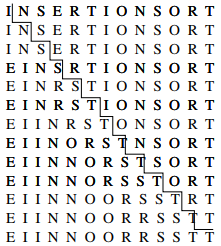
\includegraphics[scale=0.6]{./insertion_sort.png}
  \label{fig:demo-diagram}
  \caption{Animation of insertion sort in action (time flows down)}
\end{figure}


\begin{verbatim}
insertion_sort(item s[], int n)
{
    int i,j; /* counters */

    for (i=1; i<n; i++) {
        j=i;
        while ((j>0) && (s[j] < s[j-1])) {
            swap(&s[j], &s[j-1]);
            j = j-1;
        }
    }
}
\end{verbatim}

\noindent\rule{\textwidth}{0.4pt}


\begin{figure}[H]
  \centering
     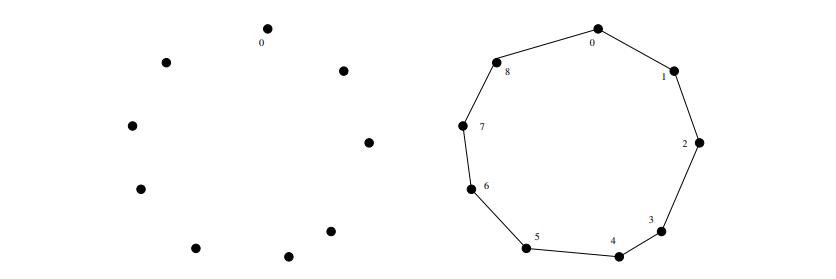
\includegraphics[scale=0.6]{./nearest_neighbor.png}
  \label{fig:demo-diagram2}
  \caption{A good instance for the nearest neighbor heuristic}
\end{figure}



